\section{Neural Networks}
\subsection{Task 3: Theory}

\subsubsection*{a)}
The binary operation XOR, or exclusive or, cannot be represented by a single-layer neural network. If we look at the two binary input values as the two digits of a binary number, we get the range $[0, 3]$. Then applying the XOR function for this range, we get $[0, 1, 1, 0]$, which obviously cannot be represented by a linear function. 

\subsubsection*{b)}
A hyperparameter is a parameter which is set before, and not changed by, the learning process. Batch size and learning rate are examples of hyperparameters. 

\subsubsection*{c)}
The softmax function is a smooth approximation of the arg max function. The values being applied to the are shifted into the range $[0, 1]$, so that they can be interpreted as probabilities, and further as a probability density function, where the sum of the result is 1. 

\subsubsection*{d)}
\begin{equation}
    \label{eq:cost_function}
    C(y_n, \hat{y}_n) = (y_n - \hat{y}_n)^2, \hat{y}_n = 1
\end{equation}

Using \cref{eq:cost_function}, we calculate: 
\begin{align*}
        w_1' = \frac{ \partial C}{\partial w_1} 
    &= \frac{\partial C}{\partial y} \frac{\partial y}{\partial c_1} 
    \frac{\partial c_1}{\partial a_1} \frac{\partial a_1}{\partial w_1}
    = 2 * (y_n - \hat{y}_n) * 1 * 1 * w_1 = - 2 * (y_n - 1) \\
        w_2' = \frac{\partial C}{\partial w_2} 
    &= \frac{\partial C}{\partial y} \frac{\partial y}{\partial c_1} 
    \frac{\partial c_1}{\partial a_2} \frac{\partial a_2}{\partial w_2}
    = 2 * (y_n - \hat{y}_n) * 1 * 1 * w_2 = 2 * (y_n - 1) \\
        w_3' = \frac{\partial C}{\partial w_3} 
    &= \frac{\partial C}{\partial y} \frac{\partial y}{\partial c_2} 
    \frac{\partial c_2}{\partial a_3} \frac{\partial a_3}{\partial w_3}
    = 2 * (y_n - \hat{y}_n) * 1 * 1 * w_3 = - 2 * (y_n - 1) \\
        w_4' = \frac{\partial C}{\partial w_4} 
    &= \frac{\partial C}{\partial y} \frac{\partial y}{\partial c_2} 
    \frac{\partial c_2}{\partial a_4} \frac{\partial a_4}{\partial w_4}
    = 2 * (y_n - \hat{y}_n) * 1 * 1 * w_4 = - 4 * (y_n - 1) \\
        b_1' = \frac{\partial C}{\partial b_1} 
    &= \frac{\partial C}{\partial y} \frac{\partial y}{\partial c_1} 
    \frac{\partial c_1}{\partial b_1} 
    = 2 * (y_n - \hat{y}_n) * 1 * 1 = 2 * (y_n - 1) \\ 
        b_2' = \frac{\partial C}{\partial b_2}
    &= \frac{\partial C}{\partial y} \frac{\partial y}{\partial c_2} 
    \frac{\partial c_2}{\partial b_2} 
    = 2 * (y_n - \hat{y}_n) * 1 * 1 = 2 * (y_n - 1) 
\end{align*}

\subsubsection*{e)}
Calculating the current value for $y$: 
\begin{align*}
    a_1 &= 1,& a_2 &= 0,& a_3 &= 1,& a_4 &= -4 \\
    c_1 &= 2,& c_2 &= -4,& y_n  &= max(c_1, c_2) = 2
\end{align*}

\begin{equation}
    \label{eq:gradient_descent}
    \theta_{t+1} = w_t - \alpha \frac{\partial C}{\partial \theta_t}
\end{equation}

Using \cref{eq:gradient_descent} and $\alpha = 0.1$, we get: 
\begin{align*}
    w_{1, t + 1} 
    &= w_{1, t} - \alpha \frac{ \partial C}{\partial w_1} 
     = -1 - 0.1 * 2 * (2 - 1) = -1.2 \\
    w_{3, t + 1} 
    &= w_{3, t} - \alpha \frac{ \partial C}{\partial w_3} 
     = -1 - 0.1 * (- 2 * (2 - 1)) = - 0.8 \\
    b_{1, t + 1} 
    &= b_{1, t} - \alpha \frac{ \partial C}{\partial b_1} 
     = 1 - 0.1 * 2 * (2 - 1) = 0.8
\end{align*}

\subsection{Task 4: Programming}
\subsubsection*{a)}
The standard training loss can be seen \cref{fig:training_loss} and the normalized here: \cref{fig:normalized_training_loss}. 

\begin{figure}[]
    \centering
    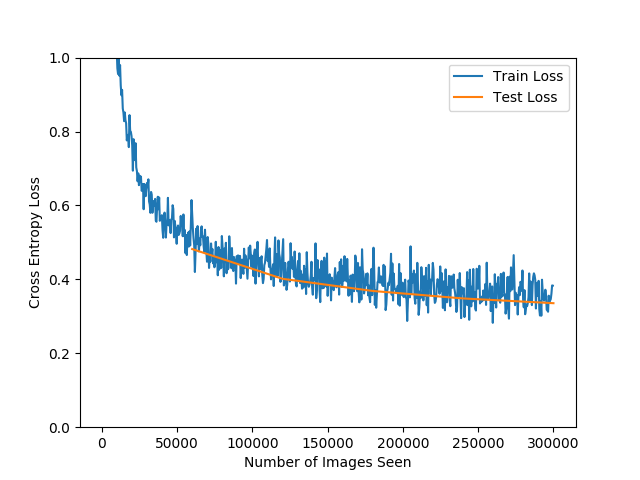
\includegraphics[width=1.00\textwidth]{figures/training_loss.png}
    \caption{Training and test loss}
    \label{fig:training_loss}
\end{figure}

\begin{figure}[]
    \centering
    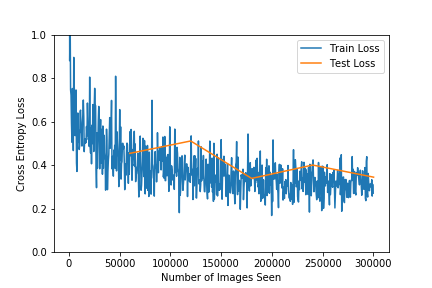
\includegraphics[width=1.00\textwidth]{figures/normalized_training_loss.png}
    \caption{Normalized training and test loss}
    \label{fig:normalized_training_loss}
\end{figure}

\subsubsection*{b)}


